\documentclass[a4paper]{article}
\usepackage{amsmath, amsthm,siunitx,amsfonts,physics}
\usepackage{tcolorbox}
\usepackage{tikz,tikz-3dplot,tikz-cd,tkz-tab,tkz-euclide,pgf,pgfplots}
\usepackage{multicol}
\tcbuselibrary{most}
\usepackage[numbers]{natbib}
\bibliographystyle{plainnat}
\usepackage{cite}
\usepackage{upgreek}
\usepackage{graphicx}
\usepackage{adjustbox}
\usepackage{url}
\usepackage{xfrac}
\graphicspath{ {./Images/} }
\usepackage[labelfont=bf]{caption}


\addtolength{\oddsidemargin}{-.45in}
\addtolength{\evensidemargin}{-.45in}
\addtolength{\textwidth}{0.9in}

\addtolength{\topmargin}{-.5in}
\addtolength{\textheight}{.385in}

\definecolor{thmcol1}{HTML}{72E094}
\definecolor{thmcol2}{HTML}{24E2D6}
\definecolor{defcol1}{HTML}{ffc500}
\definecolor{defcol2}{HTML}{c21500}
\definecolor{procol1}{HTML}{CC2B5E}
\definecolor{procol2}{HTML}{753A88}
\definecolor{corcol1}{HTML}{F29492}
\definecolor{corcol2}{HTML}{4682B4}
\definecolor{lemcol1}{HTML}{FF0000}
\definecolor{lemcol2}{HTML}{EE82EE}
\definecolor{exacol1}{HTML}{2980b9}
\definecolor{exacol2}{HTML}{0000CD}

\newtcbtheorem[number within=section]{theorem}{Theorem}%
{interior style={left color=thmcol1!15!white,right color=thmcol2!15!white},
frame style={left color=thmcol1!60!white,right color=thmcol2!60!white},coltitle=black,top=2mm,bottom=2mm,left=2mm,right=2mm,
enhanced,breakable,separator sign none}{th}

\newtcbtheorem[number within=section]{definition}{Definition}%
{interior style={left color=defcol1!15!white,right color=defcol2!15!white},
frame style={left color=defcol1!60!white,right color=defcol2!60!white},coltitle=black,top=2mm,bottom=2mm,left=2mm,right=2mm,
enhanced,breakable,separator sign none}{th}

\newtcbtheorem[number within=section]{proposition}{Proposition}%
{interior style={left color=procol1!15!white,right color=procol2!15!white},
frame style={left color=procol1!60!white,right color=procol2!60!white},coltitle=black,top=2mm,bottom=2mm,left=2mm,right=2mm,
enhanced,breakable,separator sign none}{th}

\newtcbtheorem[number within=section]{corollary}{Corollary}%
{interior style={left color=corcol1!15!white,right color=corcol2!15!white},
frame style={left color=corcol1!60!white,right color=corcol2!60!white},coltitle=black,top=2mm,bottom=2mm,left=2mm,right=2mm,
enhanced,breakable,separator sign none}{th}

\newtcbtheorem[number within=section]{lemma}{Lemma}%
{interior style={left color=lemcol1!15!white,right color=lemcol2!15!white},
frame style={left color=lemcol1!60!white,right color=lemcol2!60!white},coltitle=black,top=2mm,bottom=2mm,left=2mm,right=2mm,
enhanced,breakable,separator sign none}{th}

\newtcbtheorem[number within=section]{example}{Example}%
{interior style={left color=exacol1!15!white,right color=exacol2!15!white},
frame style={left color=exacol1!60!white,right color=exacol2!60!white},coltitle=black,top=2mm,bottom=2mm,left=2mm,right=2mm,
enhanced,breakable,separator sign none}{th}

\newenvironment{hproof}{%
  \renewcommand{\proofname}{Heuristic Proof}\proof}{\endproof}

\def\nicefrac#1#2{%
    \raise.5ex\hbox{\begin{footnotesize}$#1$\end{footnotesize}}%
    \kern-.15em/\kern-.035em%
    \lower.25ex\hbox{\begin{footnotesize}$#2$\end{footnotesize}}}

\def\Res{\text{Res}}
\def\Wind{\text{Wn}}

\begin{document}
\title{The Residue Theorem For Self-Intersecting Curves}
\author{Harvey Dhillon 2102212}
%\date{\vspace{-5ex}}
\maketitle
\thispagestyle{empty}
\clearpage
\tableofcontents
\thispagestyle{empty}
\pagebreak
\setcounter{page}{1}
\section{Introduction}


In \textit{MA244 Analysis III}, we were introduced to one of the most interesting theorems in mathematics - Cauchy's Theorem, which told us that, for a closed continuously differentiable ($\mathcal{C}^1$) curve $\gamma$ over a simply connected domain $\Omega \subseteq \mathbb{C}$, if $f: \Omega \rightarrow \mathbb{C}$ is fully analytic on $\Omega$, then $ \int_\gamma { f(\hat{z}) \dd\hat{z}} = 0$.


While this trivialises many complex contour integrals, it requires $f$ to be analytic at every point within $\Omega$, which for many functions is often not the case (for example, $f(z) = \nicefrac{1}{z}$ lacks analyticity at $z=0$). So we might ask ourselves, ``What if $f$ is not necessarily analytic at every point in $\Omega$? Are there any techniques which can help us there?'' We were later introduced to the residue theorem, which solved this dilemma:

\begin{theorem*}{(The Residue Theorem, \textit{MA244 Analysis III} Version)}{}
Let $f: \Omega \rightarrow \mathbb{C}$ be analytic on $\Omega \setminus \Phi$, where $\Omega \subset \mathbb{C}$  is open and simply connected, and $\Phi \subset \Omega$ is a closed, finite set of singularities for $f$. Let $\gamma \subset \Omega \setminus \Phi$ be a simple closed piecewise $\mathcal{C}^{1}$ curve that is oriented anticlockwise. Then 
\[ \int_\gamma { f(\hat{z}) \dd\hat{z}} = 2 \pi i \sum_{w \in \Phi}  \Res(f,w). \]
\end{theorem*}

As one of the most powerful theorems in complex analysis, the residue theorem provides a method for calculating many real and complex integrals with non-analytic points. However, the version we were introduced to has some drawbacks. It only works for simple curves and therefore does not take into account the same set of contours that can be applied to Cauchy's theorem (such as self-intersecting contours). For example, I cannot evaluate $\int_\gamma { e^{\nicefrac{1}{\hat{z}}} \dd\hat{z}}$ if $\gamma$ is an inner loop limaçon (as seen in Figure \ref{fig:limacon}) using the current residue theorem.

\begin{figure}[h!]
\begin{center}
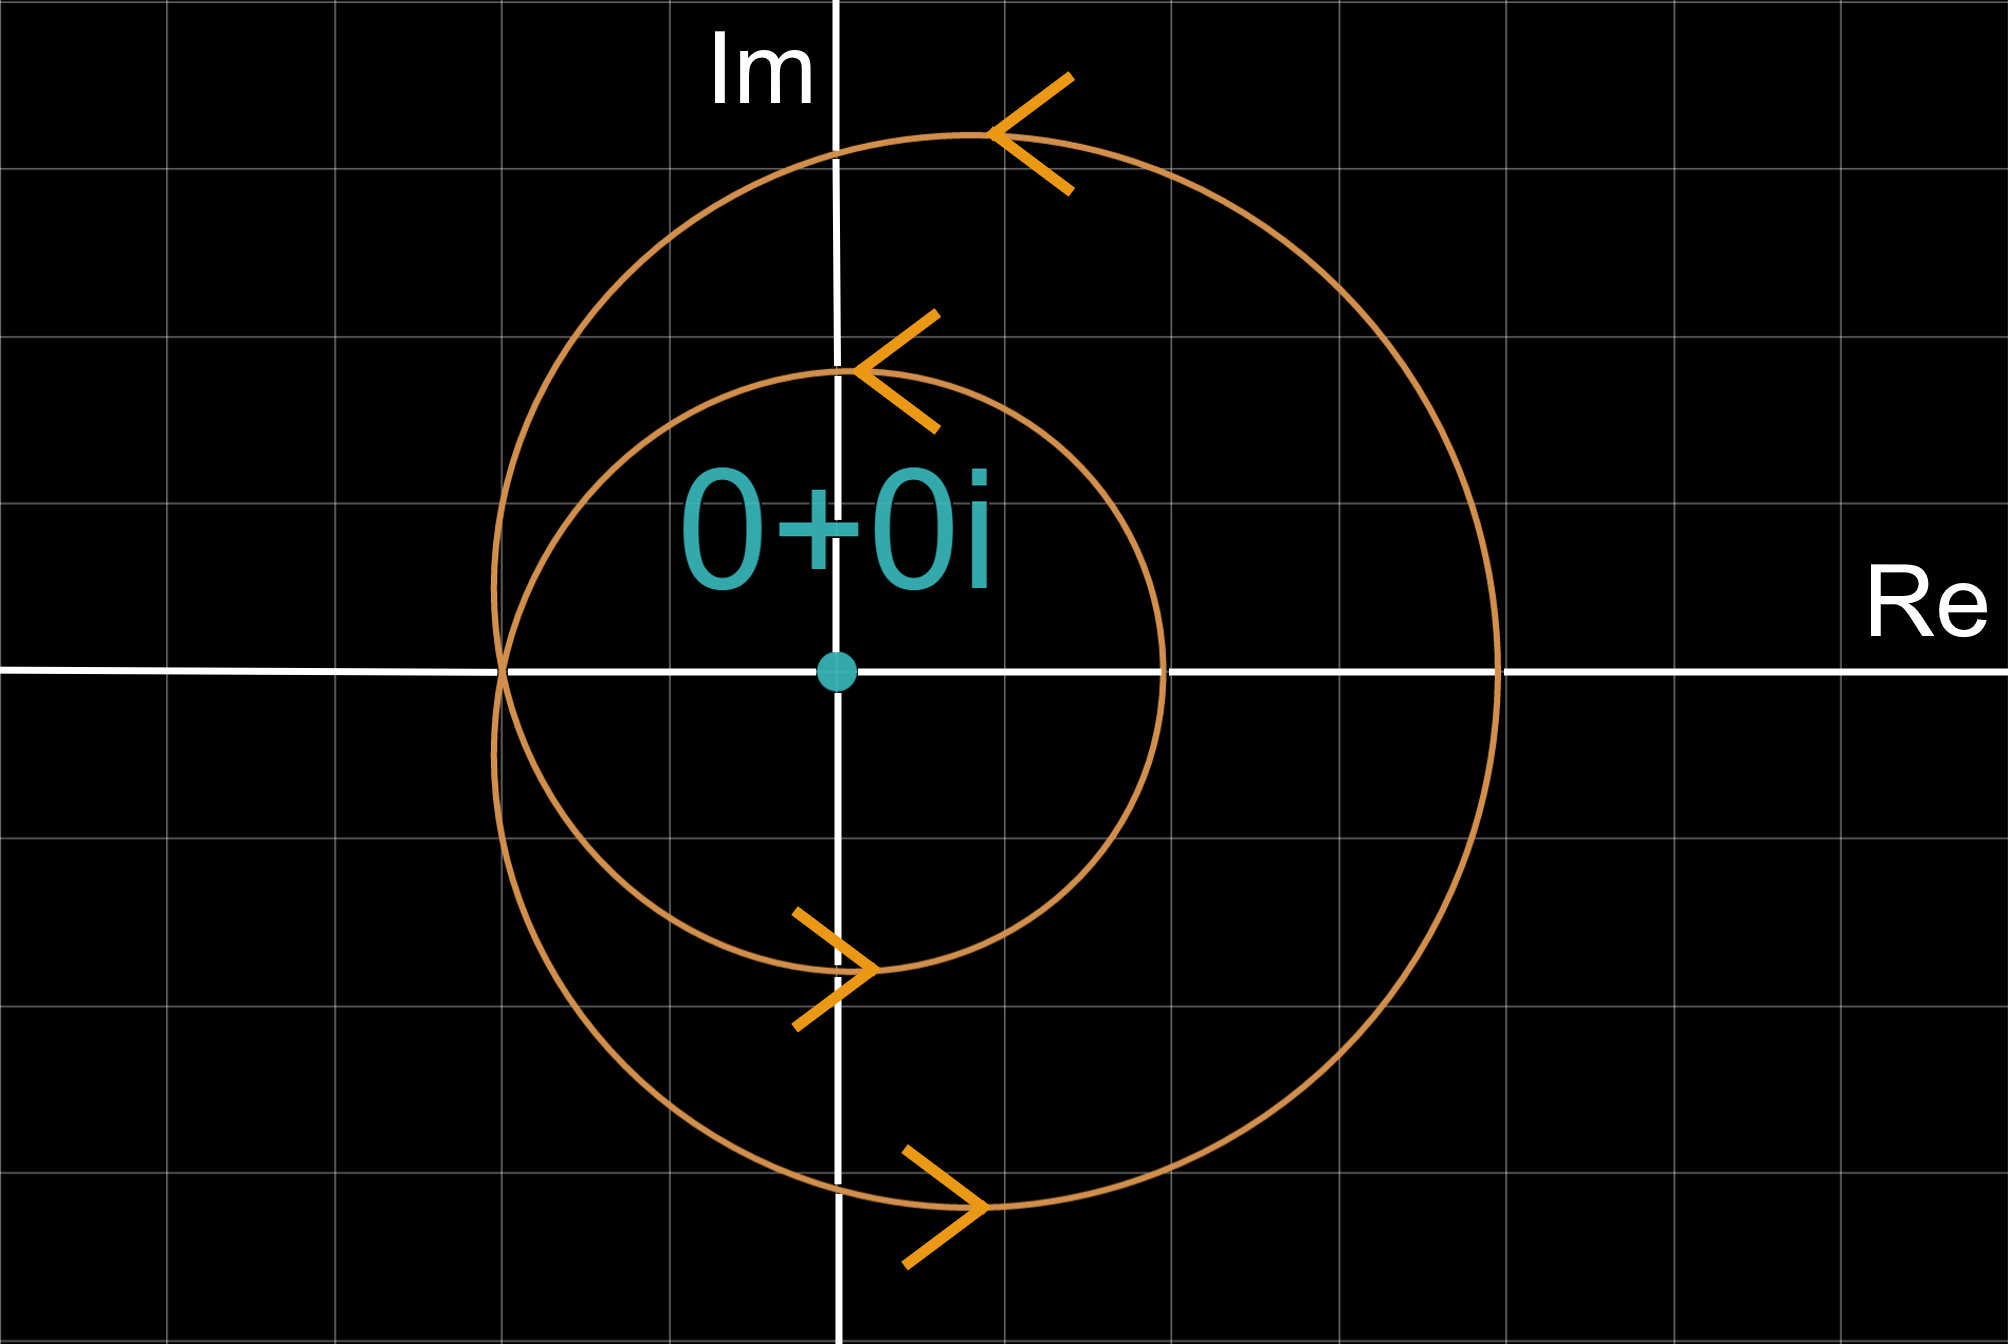
\includegraphics[scale=0.15]{limaconint3}
\end{center}
\caption{\textbf{A limaçon (an example of a self-intersecting curve)}}
\label{fig:limacon}
\end{figure}

It also assumes the set of poles is finite and not just discrete. My aim is to formulate a stronger version of the residue theorem which can be applied to any contour integral through a curve that would be sufficient for Cauchy's theorem, with a function that has discrete poles within the simply connected domain. In essence, this will be non-simple closed piecewise $\mathcal{C}^1$ curves, with any orientation. This theorem will be less limited than the version we were introduced to in \textit{MA244 Analysis III} and we will explore homotopies and winding numbers to make this possible. I also want to explore a new way of calculating residues using the Laurent series, to make calculations more efficient. To illustrate everything covered, I will gradually evaluate $\int_\gamma { e^{\nicefrac{1}{\hat{z}}} \dd\hat{z}}$ step by step through the curve shown in Figure \ref{fig:limacon} as an example.


\section{Homotopies}

We start by exploring how the deformation of curves links to the residue theorem. 

\begin{definition}{\citep[p.19]{Roe}}{}
Let $X,Y$ be metric spaces and $f,g : X \rightarrow Y$. A homotopy between $f$ and $g$ exists if there is a continuous mapping $H : X \times [0,1] \rightarrow Y $ such that $H(z,0) = f(z)$ and $H(z,1)=g(z)$.  
\end{definition}

If a homotopy connects $f$ and $g$, they are homotopic to each other. In other words, if two functions are homotopic, one can be deformed into another. For example, a circle would be homotopic to a square since they can be deformed into each other (as seen in Figure \ref{fig:circtosquare}). 
\begin{figure}[h!]
\begin{center}
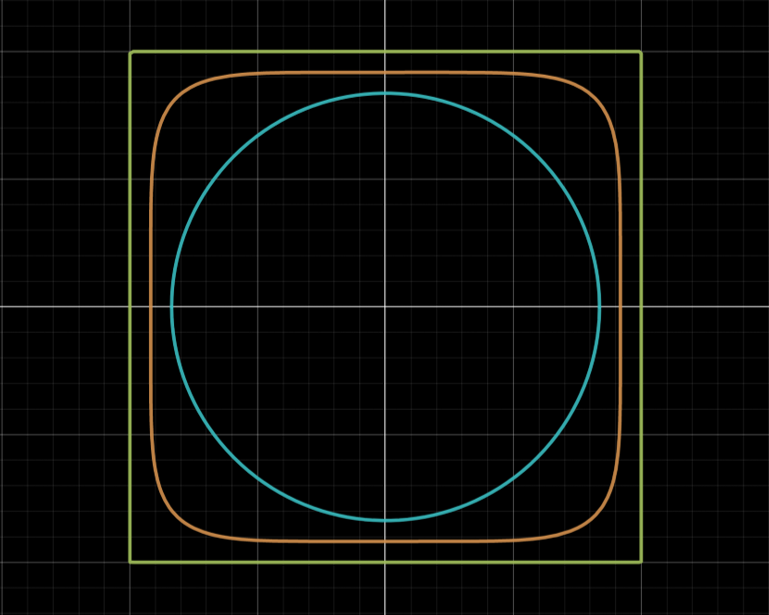
\includegraphics[scale=0.20]{c2shomotopy}
\end{center}
\caption{\textbf{How a circle can be deformed into a square}}
\label{fig:circtosquare}
\end{figure}

When a homotopy exists between $f$ and a point $w \in \mathbb{C}$, $f$ is homotopic to the constant map $g$ such that $g(z) = w$.

To visualise homotopies for closed contours, which the residue theorem requires, imagine an elastic band. The contour formed by the elastic band without any extra forces applied to it will be homotopic to the contour formed once we start stretching and manipulating it. 

The second element of the pair in the map can be thought of as a slider - as the second element travels from 0 to 1, the contour produced by $f$ will deform into the contour produced by $g$. For example, in Figure \ref{fig:circtosquare}, we can represent $H(z,0)$ by the circle, $H(z,1)$ by the square and $H(z,\alpha)$, for some $\alpha \in (0,1)$, by the contour in between.

\begin{definition}{\citep[p.22]{Roe}}{}
A set $\Omega \subset \mathbb{C}$ is simply connected if, for the set of curves $\Gamma \subset \Omega$, all $\gamma \in \Gamma$ with the same endpoints are homotopic to each other. 
\end{definition}

This is equivalent to saying all closed $\gamma \in \Gamma$ are homotopic to their endpoints in $\Omega$, since each point functions as a curve (parametrised by a constant), which is reminiscent of the definition of simply connected domains seen in \textit{MA244 Analysis III}. By defining this in terms of homotopies, it is clearer that any contour in our region $\Omega$ should be able to traverse anywhere in $\Omega$ regardless of endpoints, and there cannot be any holes in $\Omega$. 

If we consider our elastic band analogy, holes in $\Omega$ would mean we would not be able to stretch the elastic band through every  $\gamma \in \Omega$ with matching endpoints to our starting contour. Simple connectedness is necessary for the residue theorem due to the use of winding numbers, which we will explore next.

\section{Winding Numbers}

Originally conceived by August Ferdinand M{\"o}bius in 1865 (see \citep{Mobius}), the winding number, for a point $w \in \mathbb{C}$ and a curve $\gamma$, is a count of the net times a contour winds around a point anticlockwise and is denoted by $\Wind(\gamma,w)$. Before we view their effect on the residue theorem, we will rigorously define winding numbers.

\subsection{Lifting}

To intepret winding numbers mathematically, we want to build a function which observes the rotation of a contour. In order to do this, we shall investigate the process of lifting.

\begin{definition}{\citep[p.27]{Roe}}{}
Let $X$ be a metric space. A continuous map $f : X \rightarrow \mathbb{C}\setminus\{0\}$ lifts through the exponential map if there is a map $g : X \rightarrow \mathbb{C}$  such that $f = e^{g}$. 
\end{definition}

Lifting is a formalisation of the idea that we can find a composition such that $f$ can be defined continuously in terms of $h \circ g$. In this case, we use $h(z) = e^{z}$ as the map being lifted through.

\adjustbox{scale=2,center}{%
    \begin{tikzcd}
    X \arrow{d}[swap]{g} \arrow{r}{f} &Z \\
    Y \arrow{ru}[swap]{h} &{}
    \end{tikzcd}
}

This commutative diagram visualises lifting (and the rising nature of the diagram is also why it is referred to as lifting). In this case $Y$ and $Z$ refer to $\mathbb{C}$ and $\mathbb{C}\setminus \{0\}$ respectively, while $h$ refers to the exponential map.  

\begin{proposition}{\citep[p.29]{Roe}}{}
Let $\gamma :[a,b] \rightarrow \mathbb{C}\setminus\{0\}$ be a continuous path. Then $\gamma$ lifts through the exponential map to a path $\theta: [a,b] \rightarrow \mathbb{C}$.

\end{proposition}

\begin{hproof}
Let $H(t,k) = \gamma (t(1-k))$. This is a homotopy between the constant map since $H(t,0) = \gamma (t)$ and $H(t,1) = \gamma (0)$ which is a constant path. Using the fact that $f$ lifts through the exponential map if and only if $f$ is homotopic to a constant map (which can be shown using covering spaces, an advanced topological concept) we can show that $\gamma(t)$ lifts through the exponential map.
\end{hproof}

Since covering spaces are outside the scope of this essay, I have left this as a heuristic proof. Regardless, we now have the tools to create a function that separates distance from rotation for complex contours.

\newpage

\subsection{Interpreting Winding Numbers}

Using lifting, we can now form an exponential representation of a continuous contour.

\begin{lemma}{\citep[p.29]{Roe}}{} \label{thm:lifted}
Let $\gamma :[a,b] \rightarrow \mathbb{C}\setminus\{w\}$ be a continuous path. Then there exist continuous functions $\theta, r: [a,b] \rightarrow \mathbb{R}$ such that $\gamma(t) = |r(t)|e^{i\theta(t)} + w$ for all $ t \in [a,b]$.

\end{lemma}

This lemma is possible since every $\gamma : [a,b] \rightarrow \mathbb{C}\setminus\{w\}$ lifts through the exponential map to a function $\theta$. We account for the fact that the curve does not cross through $w$ by adding $w$ to our parametrisation, which centres the rotation around $w$ rather than $0$. If $w=0$ then $|r(t)| = |\gamma(t)|$ clearly as the distance of each point of $\gamma$ from $0$ will be the same as the respective distance from $r$. 

But why is it useful to parametrise $\gamma: [a,b] \rightarrow \mathbb{C}\setminus\{w\}$ as $\gamma(t) = |r(t)|e^{i\theta(t)}+w$, $t \in [a,b]$? Separating the distance from direction is important as it allows us to focus on $e^{i\theta(t)}$ in isolation. Since this only affects the rotation of the path on the complex plane, as $t$ travels from $a$ to $b$, $\theta(t)$ must describe the revolutions of the whole path. We can use this to mathematically describe the winding number.

\begin{definition}{(The Winding Number) \citep[p.30]{Roe}}{}
Let $\gamma$ : $[a,b] \rightarrow \mathbb{C}\setminus\{w\}$ be a continuous path such that $\gamma(t) = |r(t)|e^{i\theta(t)} + w$ for all $ t \in [a,b]$. Then the winding number of $\gamma$ around $w$ is
\[ \Wind(\gamma,w)   = \frac{1}{2\pi}(\theta(b) - \theta(a)). \] 

\end{definition}

Why do winding numbers affect the residue theorem though? Recall that the result of a contour integral can represent work done by that vector field - which in this case is a complex function (see \citep[p.474-476]{Needham}). Then the contour winding around a point anticlockwise $n$ times would mean that $n$ times the amount of energy needs to be transferred to circulate that point (or $-n$ if the contour is winding clockwise) so the value of the integral needs to be multiplied by the winding number. 

By Cauchy's Theorem, we know that the work done around a fully analytic function is $0$, so the only points which will require energy transfer are the singularities (points which lack analyticity) - when we form our new version of the residue theorem we are going to have to multiply these points by their winding number.


\subsection{Calculating Winding Numbers}

We are now going to explore two methods for computing winding numbers.

With a visualisation of a closed contour, we can easily compute the winding number around a point. After selecting the point to wind around, we trace through the contour $\gamma$ from $\gamma(a)$ to $\gamma(b)$; every anticlockwise rotation of $2\pi$ around the point increments the winding number and clockwise rotations decrement the value. 

In essence, this method is a simplification of the notion of the winding number as the net number of revolutions (see \citep[p.338]{Needham}). To visualise this, imagine there is a tree at the point with one end of a rope attached to it and the other end held by a person. This individual walks through the contour until they reach their original position, still holding their end of the rope. The number of times the rope has wrapped around the tree is the absolute value of the winding number, and the direction of the curls tells you which sign precedes the value (anticlockwise winds result in a positive winding number and the converse is true for clockwise winds).

But this brings up some questions: what happens if we cannot see a visualisation of the contour? Or if the visualisation is too complicated to trace through by hand? The above method works for simple cases but is not the most rigorous method for determining winding numbers. However, in such cases, the following integral can be used to calculate the number of revolutions around a point:

\begin{theorem}{\citep[p.115]{Ahlfors}}{} \label{thm:windingnumberint}
 Let $w \in \mathbb{C}$ and $\gamma: [a,b] \rightarrow \mathbb{C} \setminus \{w\}$ be a closed piecewise $\mathcal{C}^{1}$ curve. Then
\[ \Wind (\gamma,w) =\frac{1}{2\pi i} \int_{\gamma} { \frac{1}{\hat{z}-w} \dd \hat{z}}. \] 

\end{theorem}

Here we are limiting ourselves to $\mathcal{C}^{1}$ curves, so we will have to implement this restriction when we form the residue theorem.

\begin{proof}
Since $\gamma $ is a closed piecewise $\mathcal{C}^{1}$ curve, it is true that
\begin{equation}\label{eq:windint}
\int_\gamma { \frac{1}{\hat{z}-w} \dd \hat{z}} = \int_a^b { \frac{\gamma'(t)}{\gamma(t)-w} \dd t}.
\end{equation} 
Since $\gamma$ is a $\mathcal{C}^{1}$ curve, $\theta(t)$ must be $\mathcal{C}^{1}$ too, by Proposition 3.1. Then
\[\gamma(t) = |r(t)|e^{i\theta(t)}+w \implies \gamma'(t) = \dv{t} (|r(t)|e^{i\theta(t)}+w) = |r(t)|i\theta'(t)e^{i\theta(t)} + e^{i\theta(t)}\dv{t} (|r(t)|).\]
We can write the right hand side integral in (\ref{eq:windint}) as
\[\int_a^b { \frac{\gamma'(t)}{\gamma(t)-w} \dd t} = \int_a^b { \frac{|r(t)|i\theta'(t)e^{i\theta(t)} + e^{i\theta(t)}\dv{t} (|r(t)|)}{|r(t)|e^{i\theta(t)}} \dd t} =
\int_a^b { i\theta'(t)+\frac{\dv{t} (|r(t)|)}{|r(t)|}}\dd t.\]
Since 
\[\frac{\dv{t} (|r(t)|)}{|r(t)|} = \dv{t} (\log(|r(t)|)),\]
we can deduce that
\[ \int_\gamma { \frac{1}{\hat{z}-w} \dd \hat{z}} = \int_a^b { i\theta'(t)+\dv{t} (\log|r(t)|)\dd t},\]
which evaluates to
\[  i\theta(b) - i\theta(a) + \log|r(b)| - \log|r(a)|.\]
Since the curve is closed, $|r(a)|=|r(b)| \implies \log|r(b)| - \log|r(a)|=0$, leaving us with
\[ i\theta(b) - i\theta(a)  = 2\pi i \Wind (\gamma,w). \qedhere \]

\end{proof} 

This is only necessary if we do not have a visualisation of our path. However, since the residue theorem is limited to closed piecewise $\mathcal{C}^1$ curves, we can move on to proving relevant facts about winding numbers.

\newpage
\begin{proposition}{\citep[p.348]{Princeton}}{}
Let $w \in \mathbb{C}$ and $\gamma: [a,b] \rightarrow \mathbb{C} \setminus \{w\}$ be a closed piecewise $\mathcal{C}^{1}$ curve. Then $\Wind (\gamma,w)$ is always an integer. 
\end{proposition}


\begin{proof}
Let
\[ f(u) = \int_a^u { \frac{\gamma'(t)}{\gamma(t)-w} \dd t}.\]
Then $f$ is continuous on [a,b] and differentiable on (a,b). By the fundamental theorem of calculus,
\begin{equation}\label{eq:derivwind1}
f'(u) =  \frac{\gamma'(u)}{\gamma(u)-w}.
\end{equation}
Take
\begin{equation}\label{eq:derivwind2}
\dv{u} (e^{-f(u)}(\gamma(u)-w)) = e^{-f(u)}\gamma'(u) - f'(u)e^{-f(u)}(\gamma(u)-w).
\end{equation}
After substituting (\ref{eq:derivwind1}) into (\ref{eq:derivwind2}) we obtain
\[e^{-f(u)}\gamma'(u) - f'(u)e^{-f(u)}(\gamma(u)-w) = e^{-f(u)}\gamma'(u) - \frac{\gamma'(u)e^{-f(u)}(\gamma(u)-w)}{\gamma(u)-w}=0,\]
so $e^{-f(u)}(\gamma(u)-w) = C$, where $C$ is a constant, implying $Ce^{f(u)} = \gamma(u)-w.$
Since $\gamma(a) = \gamma(b)$, as the curve is closed,
\[ Ce^{f(a)} = \gamma(a)-w = \gamma(b)-w = Ce^{f(b)}.\]
Since $\gamma(a)-w$ can take non-zero values, $C \neq 0$, so $e^{f(a)}=e^{f(b)}$. Therefore, the exists a $Z \in \mathbb{Z}$ such that
\[2\pi i Z = f(b) - f(a).\]
Since $f(a) = \int_a^a { \nicefrac{\gamma'(t)}{(\gamma(t)-w)} \dd t} = 0$, $2\pi i Z = f(b)$. Therefore,
\[\frac{f(b)}{2\pi i } = \frac{1}{2\pi i }\int_a^b { \frac{\gamma'(t)}{\gamma(t)-w} \dd t} = \frac{1}{2\pi i }\int_\gamma { \frac{1}{\hat{z}-w} \dd \hat{z}} =\Wind (\gamma,w) = Z. \qedhere\]
\end{proof}

If we think back to our ``rope around a tree'' visualisation, it is intuitive that the winding number would be an integer as the rope would finish off in a position which is aligned to where it started, since the endpoint matches the starting point. 

\begin{corollary}{}{} \label{thm:constantwind}
Let $\gamma$ : $[a,b] \rightarrow \mathbb{C}$ be a closed piecewise $\mathcal{C}^{1}$ curve. Then for all $w$ on each component of $\mathbb{C} \setminus \gamma([a,b])$, $\Wind (\gamma, w)$ is constant.
\end{corollary}

\begin{proof}
By the fundamental theorem of contour integrals
\[ \Wind (\gamma,w) = \int_\gamma { \frac{1}{\hat{z}-w} \dd \hat{z}} \implies \Wind '(\gamma,w) =   \frac{1}{\gamma(b)-w }-\frac{1}{\gamma(a)-w}.\]
Since the curve is closed, $\gamma(b)=\gamma(a)$, which results in $\Wind '(\gamma,w)=0$ meaning $\Wind (\gamma,w)$ must be constant in that component.
\end{proof}

This is important as it tells us that all points inside a single component will have the same winding number. However, this does not mean that the winding number is necessarily constant throughout the entirety of the complex plane. Recall that from Theorem 3.1, $\Wind (\gamma,w)$  is not defined for $w \in \gamma$, so the constancy of $\Wind (\gamma,w)$ only applies for the component it is located in. Still, this will likely save a lot of time computing winding numbers -  especially if we have a visualisation of our contour, since we only need to identify the winding number of a single point in each component to identify them all. 

Finally, we explore what happens to the winding number of points outside a closed contour.

\begin{corollary}{}{} \label{thm:unboundedwind}
Let $\gamma$ : $[a,b] \rightarrow \mathbb{C}$ be a closed and bounded piecewise $\mathcal{C}^{1}$ curve. Then for all $w$ on the unbounded component of $\mathbb{C} \setminus \gamma([a,b])$, $\Wind (\gamma, w)$ is $0$.
\end{corollary}

\begin{proof}
Inspecting
\[ \Wind(\gamma,w) = \int_\gamma { \frac{1}{\hat{z}-w} \dd \hat{z}},\]
if $w$ is not in the interior of the contour $\gamma$, $\nicefrac{1}{\hat{z}-w}$ will be analytic in the region to be integrated, so by Cauchy's Theorem
\[\int_\gamma { \frac{1}{\hat{z}-w} \dd \hat{z}} = 0 \implies \Wind (\gamma,w) = 0. \qedhere\]
\end{proof}

So any point outside a contour will have a winding number of 0 with respect to that contour. Intuitively this is obvious as a closed curve will never be able to circulate around exterior points. 
 

This is useful if $\Omega \subset \mathbb{C}$ is open and simply connected, as $\gamma \in \Omega$ will be homotopic to a point in $\Omega$, leading to no holes in $\Omega$. Therefore all $w \notin \Omega$ are guaranteed to be in the unbounded component for every closed contour $\gamma \in \Omega$, so by Corollary 3.2, for all $w \notin \Omega$, $\Wind(\gamma, w)=0$. This is why simple connectedness will be essential when proving the residue theorem.

\begin{example}{}{}
Find the winding numbers of A, B, C, D and E in the closed curve $\gamma$.

\begin{center}
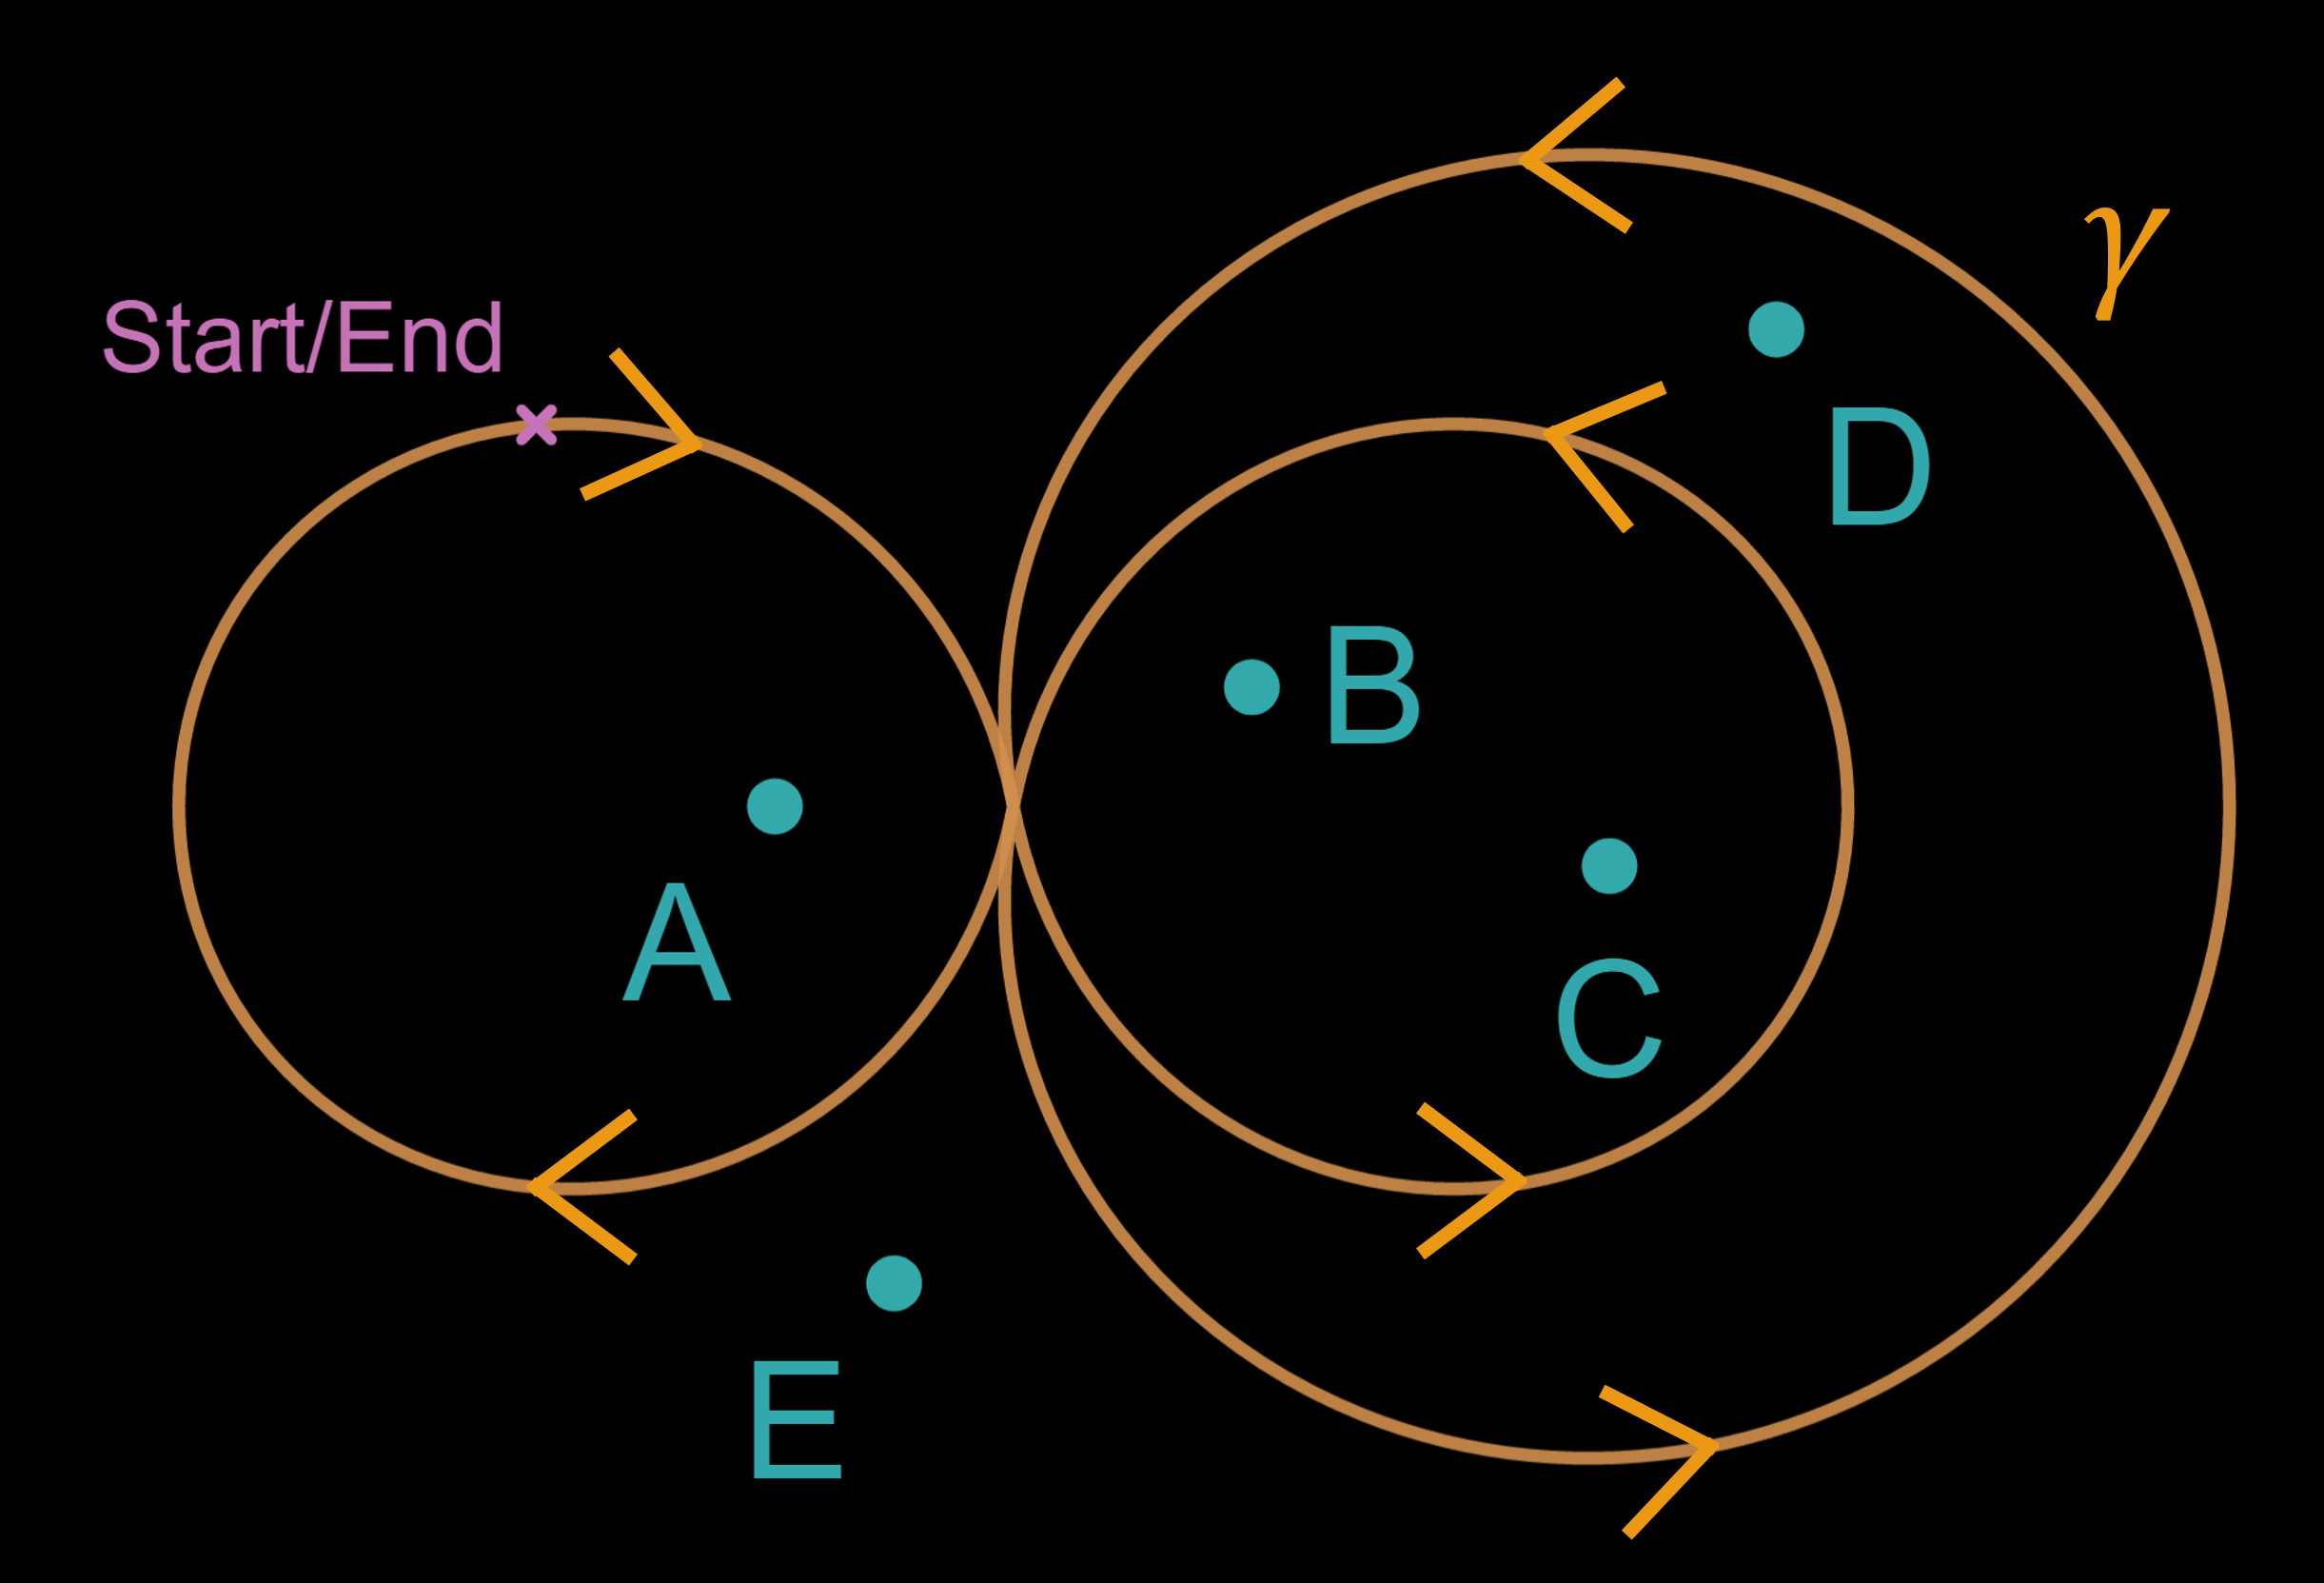
\includegraphics[scale=0.13]{windingnumbers}
\end{center}
\end{example} 

\noindent\textit{Solution.}
A: We trace the curve around and revolve around A once clockwise - $\Wind (\gamma,\text{A})=-1$.

B: We trace again and revolve twice anticlockwise around B  - $\Wind(\gamma,\text{B})=2$.

C: By Corollary 3.1, since B and C are in the same component, $\Wind (\gamma,\text{B})=W(\gamma,\text{C})=2$.

D: Again, tracing shows that the curve revolves once anticlockwise around D - $\Wind (\gamma,\text{D})=1$.

E: Since E is in the unbounded component of the curve, by Corollary 3.2, $\Wind(\gamma,\text{E})=0$.


Despite the complicated theorems and definitions, evaluating winding numbers is relatively easy, but is fundamental for applying the residue theorem through self-intersecting curves.

\newpage
\section{The Laurent Series}

As seen in \textit{MA131 Analysis II} and \textit{MA244 Analysis III}, the Taylor series can be used to represent functions as a convergent power series around a point $w$ where $B_{\upvarepsilon}(w)$ is analytic for a value of $\upvarepsilon>0$. Of course, we cannot represent partially analytic functions with finite singularities with a Taylor expansion. Fortunately, there is another way to represent these functions that we can investigate: the Laurent series. 

\begin{theorem}{(The Laurent Expansion) \citep[p.222]{Marsden}}{} \label{thm:laurentexists} 
Let $w \in \mathbb{C}$, $\Omega \subseteq \mathbb{C}$ and $f: \Omega \rightarrow \mathbb{C}$ be analytic on the region $F = \{z \in \mathbb{C} \mid r < |z-w|< s\} $ with $r,s \in \mathbb{R}$ and $0\leq r<s$ such that $F \subset \Omega$. Let, for $r< \upvarepsilon <s$,
\[a_{j} = \frac{1}{2\pi i }\int_{\partial B_{\upvarepsilon}(w)} { \frac{f(\hat{z})}{(\hat{z}-w)^{j+1}} \dd \hat{z}}.\]
Then, for all $z \in F$, the Laurent expansion of $f(z)$ at $w$ is
\[f(z) = \sum_{j \in \mathbb{Z}} a_{j}(z-w)^{j}.\]
\end{theorem}

The Laurent series was named after and published by Pierre Alphonse Laurent in 1843, but may have actually been discovered by Karl Weierstrass in 1841, only to be published after his death (see \citep[p.12]{Spirit}). 

\begin{proof}

Firstly we prove its existence. Choose $R$ and $S$ such that $r<R<|z-w|<S<s$. The integral of an analytic function around $\partial B_{\upvarepsilon}(w)$ is independent of $\upvarepsilon$ (where $r< \upvarepsilon <s$), so
\[a_{j} = \frac{1}{2\pi i }\int_{\partial B_{R}(w)} { \frac{f(\hat{z})}{(\hat{z}-w)^{j+1}} \dd\hat{z}} = \frac{1}{2\pi i }\int_{\partial B_{S}(w)} { \frac{f(\hat{z})}{(\hat{z}-w)^{j+1}} \dd\hat{z}}.\]
Using the fact that, for $z$ in the interior of $\gamma$,
\[f(z) = \frac{1}{2\pi i} \int_{\gamma} \frac{f(\hat{z})}{\hat{z}-z}\dd \hat{z},\]
we can represent the function as
\begin{align}
f(z) &=\frac{1}{2\pi i }\int_{\partial B_{S}(w)+L-\partial B_{R}(w)-L} { \frac{f(\hat{z})}{\hat{z}-z} \dd\hat{z}} \nonumber \\
& \label{eq:annuliint}=\frac{1}{2\pi i }\int_{\partial B_{S}(w)} { \frac{f(\hat{z})}{\hat{z}-z} \dd\hat{z}} - \frac{1}{2\pi i }\int_{\partial B_{R}(w)} { \frac{f(\hat{z})}{\hat{z}-z} \dd\hat{z}},
\end{align}
where $L$ is a straight line connecting the two circles together as a path, so the region encapsulated by the integral is guaranteed to be analytic. By its Taylor expansion, we know that
\[\frac{1}{2\pi i }\int_{\partial B_{S}(w)} { \frac{f(\hat{z})}{(\hat{z}-w)^{j+1}} \dd\hat{z} = \frac{f^{(j)}(w)}{j!}},\]
which is the coefficient of each element of the Taylor series. Also, we deduce that, around $w$, 
\[\frac{1}{\hat{z}-z} = \frac{1}{(\hat{z}-w)-(z-w)}= \frac{1}{(\hat{z}-w)(1-\frac{z-w}{\hat{z}-w})} =  \sum_{j=0}^{\infty}  \frac{(z-w)^{j}}{(\hat{z}-w)^{j+1}}.\]
So we can represent the first term of (\ref{eq:annuliint}) as
\[\sum_{j=0}^{\infty}\frac{(z-w)^{j}}{2\pi i }\int_{\partial B_{S}(w)} { \frac{f(\hat{z})}{(\hat{z}-w)^{j+1}} \dd\hat{z}} = \sum_{j=0}^{\infty} a_{j}(z-w)^{j}.\]
Now, for any $z \in \partial B_{R}(w)$
\[-\frac{1}{\hat{z}-z} = \frac{1}{(z-w)-(\hat{z}-w)}= \frac{1}{(z-w)(1-\frac{\hat{z}-w}{z-w})} = \frac{1}{z-w} \sum_{j=1}^{\infty} \left( \frac{\hat{z}-w}{z-w}\right) ^{j+1},\]
which is a convergent geometric series since $|\hat{z}-w| \leq R <|z-w| $, so we can represent the second term of (\ref{eq:annuliint}) as

\begin{align}
 - \frac{1}{2\pi i }\int_{\partial B_{R}(w)} { \frac{f(\hat{z})}{\hat{z}-z} \dd\hat{z}} 
 &= \frac{1}{2\pi i }\int_{\partial B_{R}(w)} \frac{1}{z-w} \sum_{j=1}^{\infty} f(\hat{z}) \left( \frac{\hat{z}-w}{z-w}\right) ^{j+1}\dd\hat{z} \nonumber \\
 & =\sum_{j=-\infty}^{-1}\frac{1}{2\pi i }\int_{\partial B_{R}(w)} \frac{1}{z-w} f(\hat{z}) \left( \frac{z-w}{\hat{z}-w}\right) ^{j+1}\dd\hat{z} \nonumber \\
& = \sum_{j=-\infty}^{-1}\frac{(z-w)^{j}}{2\pi i }\int_{\partial B_{R}(w)}   \frac{f(\hat{z})}{(\hat{z}-w) ^{j+1}}\dd\hat{z} \nonumber \\ 
& \label{eq:principalconverges}=\sum_{j=-\infty}^{-1} a_{j} (z-w)^{j}. 
\end{align}
Now, if we replace both terms in (\ref{eq:annuliint}), we see that
\[f(z) = \sum_{j=0}^{\infty} a_{j}(z-w)^{j}+ \sum_{j=-\infty}^{-1} a_{j} (z-w)^{j}= \sum_{j \in \mathbb{Z}} a_{j}(z-w)^{j},\]
which proves the existence of the Laurent expansion.

Next, we will prove uniqueness of the Laurent expansion. Take $f(z)$ from Theorem 4.1. Since $f$ is convergent in $F$, we can divide by $(z-w)^{k+1}$ to produce
\begin{equation}\label{eq:unqlaurent} \frac{f(z)}{(z-w)^{k+1}} = \sum_{j \in \mathbb{Z}} a_{j}(z-w)^{j-k-1}, \end{equation}
which will also be convergent.
From \textit{MA244 Analysis III}, we know that
\begin{equation}\label{eq:minus1integral} \int_{\partial B_{\upvarepsilon}(w)}(\hat{z}-w)^{j}\dd\hat{z}= \begin{cases} 2\pi i & \text{if } j=-1 , \\ 0 & \text{otherwise.} \end{cases} \end{equation}
If we take (\ref{eq:unqlaurent}) and integrate the summation term by term, we obtain
\begin{align}\sum_{j \in \mathbb{Z}} \int_{\partial B_{\upvarepsilon}(w)} a_{j}(\hat{z}-w)^{j-k-1} \dd\hat{z} &= \dotsb + 0 + \int_{\partial B_{\upvarepsilon}(w)} a_{k}(\hat{z}-w)^{-1} \dd\hat{z} + 0 + \dotsb \nonumber \\
&= 2\pi i a_{k}, \nonumber 
\end{align}
since each term evaluates to 0 except when $j = -1$. Since this is true for all $k \in \mathbb{Z}$, the coefficient $a_{k}$ must be uniquely determined by $f(z)$, so the Laurent expansion is uniquely determined by $f(z)$.
\end{proof}

Since we will use the Laurent expansion to compute residues which are dependent on the function, its uniqueness for each function is necessary. The Laurent series has a lot in common with the Talyor series in that regard - in fact it is clear that all positive power terms form a Taylor series expansion. Furthermore, it is useful to isolate the infinite polynomial from the negative power terms:
\begin{definition}{\citep[p.75]{Princeton}}{}
If the Laurent expansion of $f$ at $w$ is given by
\[f(z) = \sum_{j \in \mathbb{Z}} a_{j}(z-w)^{j}\]
then the principal part of $f$ at $w$ is
\[\mathcal{P}(f,w) = \sum_{j=-\infty}^{-1} a_{j}(z-w)^{j}.\]
\end{definition}

The principal part of the Laurent expansion $\mathcal{P}(f,w)$ contains all terms of the Laurent expansion that are not analytic for all $w \in \mathbb{C}$, since the rest of the terms of the Laurent expansion form a power series. This implies that, for a closed discrete set $\Phi$ containing all singularities of $f$ then
\begin{equation}\label{eq:principalremoved}
f(z) - \sum_{w_{res}\in\Phi}\mathcal{P}(f,w_{res})
\end{equation}
is analytic for all $w \in \mathbb{C}$. This will be relevant when proving the residue theorem since, assuming the other conditions of Cauchy's theorem apply, the contour integral of (\ref{eq:principalremoved}) will evaluate to $0$.

To illustrate the Laurent series, we shall compute an expansion:

\begin{example}{}{}\label{thm:explaurentexpansion}
Define $f: \mathbb{C}\setminus\{0\} \rightarrow \mathbb{C}$ by $f(z)=e^{\nicefrac{1}{z}}.$ Compute the coefficients of the Laurent series 
\[f(z) = \sum_{j \in \mathbb{Z}} a_{j}z^{j}.\]
\end{example} 

\noindent\textit{Solution.}
Essentially we need to evaluate the Laurent series of $f(z)$ around $0$. The integral
\[\frac{1}{2\pi i }\int_{\partial B_{\upvarepsilon}(0)} { \frac{e^{\nicefrac{1}{\hat{z}}}}{(\hat{z})^{j+1}} \dd \hat{z}}\text{, }  j \in \mathbb{Z}\]
is quite complicated to solve using integration methods. But we can derive a Laurent expansion for $f(z)$ from the Taylor series for $e^{z}$ at $0$ by substituting $z$ for $\nicefrac{1}{z}$:
\[e^{z} = \sum_{j=0}^{\infty} \frac{z^{j}}{j!} \implies e^{\nicefrac{1}{z}} = \sum_{j=0}^{\infty} \frac{(\nicefrac{1}{z})^{j}}{j!} = \sum_{j=0}^{\infty} \frac{{z}^{-j}}{j!} = \sum_{j=-\infty}^{0} \frac{{z}^{j}}{(-j)!}.\]
This gives us the Laurent expansion of $f(z)$. We can observe that the coefficients of the Laurent expansion at 0, denoted $a_{j}$, are 
\begin{equation} \label{eq:coefficientslaurent}
a_{j}=\begin{cases} \nicefrac{1}{(-j)!}, & \text{if } j\leq 0 , \\ 0, & \text{otherwise.} \end{cases} 
\end{equation}

\section{The Residue Theorem}

We are finally ready to approach the residue theorem and assemble the tools we have established so far - the final step before that is defining and computing residues.

\subsection{Residues}



\begin{definition}{(Residues) \citep[p.5]{Mitrinovic}}{} \label{thm:residuedef}
Let $w \in \mathbb{C}$, $\Omega \subseteq \mathbb{C}$ and $f: \Omega \rightarrow \mathbb{C}$ be analytic on the region $F = \{z \in \mathbb{C} \mid r < |z-w|< s\} $ with $r,s \in \mathbb{R}$ and $0\leq r<s$ such that $F \subset \Omega$. Then, for $r< \upvarepsilon <s$, the residue of $f$ at $w$ is
\[\Res (f,w) = \frac{1}{2\pi i}\int_{\partial B_{\upvarepsilon}(w)} f(\hat{z}) \dd \hat{z}.\]

\end{definition}

Essentially, each residue is the integral of $f(z)$ around a singularity, through a contour where the rest of the interior is analytic. If the singularities are discrete, we can find $\upvarepsilon$ such that the ball $B_{\upvarepsilon}(w)$ is always in an analytic region for $f$. The actual value of $\upvarepsilon$ does not matter besides it being within the range $r< \upvarepsilon <s$ - the integral of $f(z)$ will be independent of $\upvarepsilon$ while on the analytic region.

Computing the contour integral directly to calculate residues might be difficult - the Laurent series can simplify this:

\begin{lemma}{\citep[p.5]{Mitrinovic}}{}
If the Laurent expansion of $f$ at $w$ is given by
\[f(z) = \sum_{j \in \mathbb{Z}} a_{j}(z-w)^{j},\]
then 
\[\Res (f,w) = a_{-1}.\]

\end{lemma}

\begin{proof}
Using Definition 5.1 and that $f(z) = \sum_{j \in \mathbb{Z}} a_{j}(z-w)^{j}$, 
\begin{align}
\Res(f,w) &=\frac{1}{2\pi i}\int_{\partial B_{\upvarepsilon}(w)} f(\hat{z}) \dd \hat{z} \nonumber \\
& = \frac{1}{2\pi i}\int_{\partial B_{\upvarepsilon}(w)} \sum_{j \in \mathbb{Z}} a_{j}(\hat{z}-w)^{j} \dd \hat{z} \nonumber \\
& \label{eq:sumofintlaurent} = \sum_{j \in \mathbb{Z}} \frac{a_{j}}{2\pi i}\int_{\partial B_{\upvarepsilon}(w)} (\hat{z}-w)^{j} \dd \hat{z} 
\end{align}
By (\ref{eq:minus1integral}), we know all the terms of (\ref{eq:sumofintlaurent}) will evaluate to $0$ except when $j=-1$, so the result will be 
\[ \dotsb + 0 + \frac{a_{-1}}{2\pi i}\int_{\partial B_{\upvarepsilon}(w)} (\hat{z}-w)^{-1} \dd \hat{z} + 0 + \dotsb = a_{-1}. \qedhere \]
\end{proof}

So if we know the Laurent expansion for $f(z)$ around singularity $w$ then we can deduce that the residue of a point $w$ is the coefficient $a_{-1}$ - the following example highlights how efficient this can be for complicated integrals.


\begin{example}{}{}\label{thm:expresexample}
Define $f: \mathbb{C}\setminus\{0\} \rightarrow \mathbb{C}$ by $f(z)=e^{\nicefrac{1}{z}}.$ Compute the residues of $f(z)$.
\end{example} 
\noindent\textit{Solution.}
We look for values of $z$ which are singularities for $f(z)$. Clearly, $f(z)$ only lacks analyticity at $z=0$, so we consider the residue at $f(0)$ and attempt to compute $\Res (f,0)$. Rather than struggling to compute the integral
\[\frac{1}{2\pi i}\int_{\partial B_{\upvarepsilon}(0)} e^{\nicefrac{1}{\hat{z}}} \dd \hat{z},\]
we can look at the coefficients of the Laurent expansion of $f(z)$ which we evaluated in Example 4.1. Using (\ref{eq:coefficientslaurent}) and setting $j=-1$, we can deduce that
\[a_{-1} = \frac{1}{1!} = 1\]
and so $\Res (f,0)=1$. Since there are no other singularities, we are done.

It should now be clear that the Laurent series is incredibly helpful when calculating residues. Now that we have explored winding numbers and residues, we are able to construct a stronger version of the residue theorem. 

\subsection{Proof of the Residue Theorem}
\begin{theorem}{(The Residue Theorem) \citep[p.133-134]{Bak}}{} \label{thm:resthm}
Let $f: \Omega \rightarrow \mathbb{C}$ be analytic on $\Omega \setminus \Phi$, where $\Omega \subseteq \mathbb{C}$  is open and simply connected, and $\Phi \subset \Omega$ is a closed, discrete set of singularities for $f$.


Let $\gamma \subset \Omega \setminus \Phi$ be a closed piecewise $\mathcal{C}^{1}$ curve. Then 
\[ \int_\gamma { f(\hat{z}) \dd\hat{z}} = 2 \pi i \sum_{w \in \Phi} \Wind (\gamma,w) \Res (f,w). \]

\end{theorem}

The residue theorem requires some conditions to be in place. Firstly, $f$ can only have a discrete set of singularities, as it must be necessary to create an analytic region around each of them for their residue to be calculated - having a continuous set of singularities would prevent us from creating analytic regions even with an infinitesimally small radius. Secondly, our coverage of the winding number has restricted the contours we can integrate through to be closed $\mathcal{C}^{1}$ curves. Finally $\Omega$ being simply connected ensures that the winding number of any singularities outside $\Omega$ is $0$.

\begin{proof}
Let $\phi = \{ w \in  \Phi \mid \Wind (\gamma,w) \neq 0\}$. 

If $\phi$ is not finite, we can pick a sequence $w_{n} \in \phi$ with pairwise distinct elements. $\phi$ is bounded, so there is a subsequence $w_{n_{j}} \rightarrow w$, $w \in \overline{\Omega}$.

If $w \in \Omega$, then $w \in \Phi$, which would mean that for all $\upvarepsilon > 0  $, there exists $N_{A}$ such that, for $n_{j} \geq N_{A}$, $w_{n_{j}} \in B_{\upvarepsilon}(w)$. This is impossible as $\Phi$ is a closed, discrete set.

Since $w_{n_{j}} \in \Omega$, which is open, $w \in \partial \Omega$ as this is the only possible region $w_{n_{j}}$ could converge to.

Since $\Omega$ is a simply connected domain, $\gamma$ (being a closed curve) is homotopic to a $w \in \Omega$, meaning any point $w \notin \Omega$ leads to $\Wind (\gamma,w)=0$, by Corollary 3.2, since it is clearly in the unbounded component of the curve. Since the winding number in each component is constant, there exists $N_{B}$ such that for all $n_{j} \geq N_{B} $, $w_{n_{j}}$ is outside of $\gamma$. Therefore, when $n_{j} \geq N_{B}$, $w_{n_{j}}$ is in the same component as $w$. By Corollary 3.1, those elements of the subsequence must also have a winding number of $0$, which contradicts $w_{n_{j}} \in \phi$ for all $w_{n_{j}}$. 

So the amount of elements in $\phi$ must be finite. Now that we know there are a finite amount of singularities, we will show the effect of them on the value of the integral. For each $w_{res} \in \phi$, note $\mathcal{P}(f,w_{res})$ is analytic for $\mathbb{C}\setminus \{w_{res}\}$, since $\mathcal{P}(f,w_{res})$ is convergent in that region, as proven in (\ref{eq:principalconverges}). 

Similarly, it is clear that $f(z) - \mathcal{P}(f,w_{res})$ is analytic at $w_{res}$ as it can be represented by a power series now that we have removed the principal part, and $f(z) - \mathcal{P}(f,z)$ is defined for any $z\in\mathbb{C}$. Therefore
\[f(z) - \sum_{w_{res}\in\phi}\mathcal{P}(f,w_{res})\]
must be analytic all throughout $\Omega$.
By Cauchy's Theorem,
\[\int_{\gamma}f(\hat{z}) - \sum_{w_{res}\in\phi}\mathcal{P}(f,w_{res})\dd\hat{z}=0 \implies \int_{\gamma}f(\hat{z}) \dd\hat{z}= \int_{\gamma}\sum_{w_{res}\in\phi}\mathcal{P}(f,w_{res})\dd\hat{z}.\]
For any $w_{res}\in\phi$, we have
\begin{equation}\label{eq:principalreverse}\int_{\gamma}\mathcal{P}(f,w_{res})\dd\hat{z} = \int_{\gamma}\sum_{j=-\infty}^{-1} a_{j}(\hat{z}-w_{res})^{j}\dd\hat{z}. \end{equation}
By (\ref{eq:minus1integral}), we know all terms of (\ref{eq:principalreverse}) will vanish besides the case where $j=-1$, so 
\[\int_{\gamma}\mathcal{P}(f,w_{res})\dd\hat{z} = a_{-1}\int_{\gamma} \frac{1}{\hat{z}-w_{res}}\dd\hat{z}  = 2\pi i \Wind (\gamma,w_{res}) \Res (f,w_{res}).\]
So, 
\begin{align}
\int_{\gamma}\sum_{w_{res}\in\phi}\mathcal{P}(f,w_{res})\dd\hat{z} &= \sum_{w_{res}\in\phi}\int_{\gamma}\mathcal{P}(f,w_{res})\dd\hat{z} \nonumber \\
&\label{eq:phiresthm}=2\pi i \sum_{w_{res}\in\phi} \Wind (\gamma,w_{res}) \Res (f,w_{res}),
\end{align}
and for $w \in \Phi \setminus \phi$, we know $\Wind (\gamma,w)=0$, so we can extend (\ref{eq:phiresthm}) to
\[\int_{\gamma}f(\hat{z}) \dd\hat{z}=2 \pi i \sum_{w\in\Phi}\Wind (\gamma,w) \Res (f,w),\]
proving the residue theorem.
\end{proof}

Dissecting the proof, we can observe that, unlike the version of the residue theorem we were introduced to in \textit{MA244 Analysis III}, we only need the set of singularities to be discrete, not finite - because the simply connected domain ensures that the winding number of the singularities will eventually be 0 for a given contour since our domain is open. 

We can also notice that the summation of residues multiplied by winding numbers is solely determined by the principal part of the Laurent expansion of the given function, which means that the power series component has no bearing on the residue theorem, which follows from Cauchy's theorem.

\subsection{The Residue Theorem in Action}

Now that we have established the residue theorem, let us return to our example from earlier, which is difficult to integrate by conventional integration methods, but is straightforward to evaluate with the residue theorem. 


\begin{example}{}{}\label{thm:finalexample}
Compute
\[ \int_\gamma { f(\hat{z}) \dd\hat{z}}\]
where $f: \mathbb{C}\setminus\{0\} \rightarrow \mathbb{C}$ is defined by $f(z)=e^{\nicefrac{1}{z}}$ and $\gamma$ is represented by the contour below.

\begin{center}
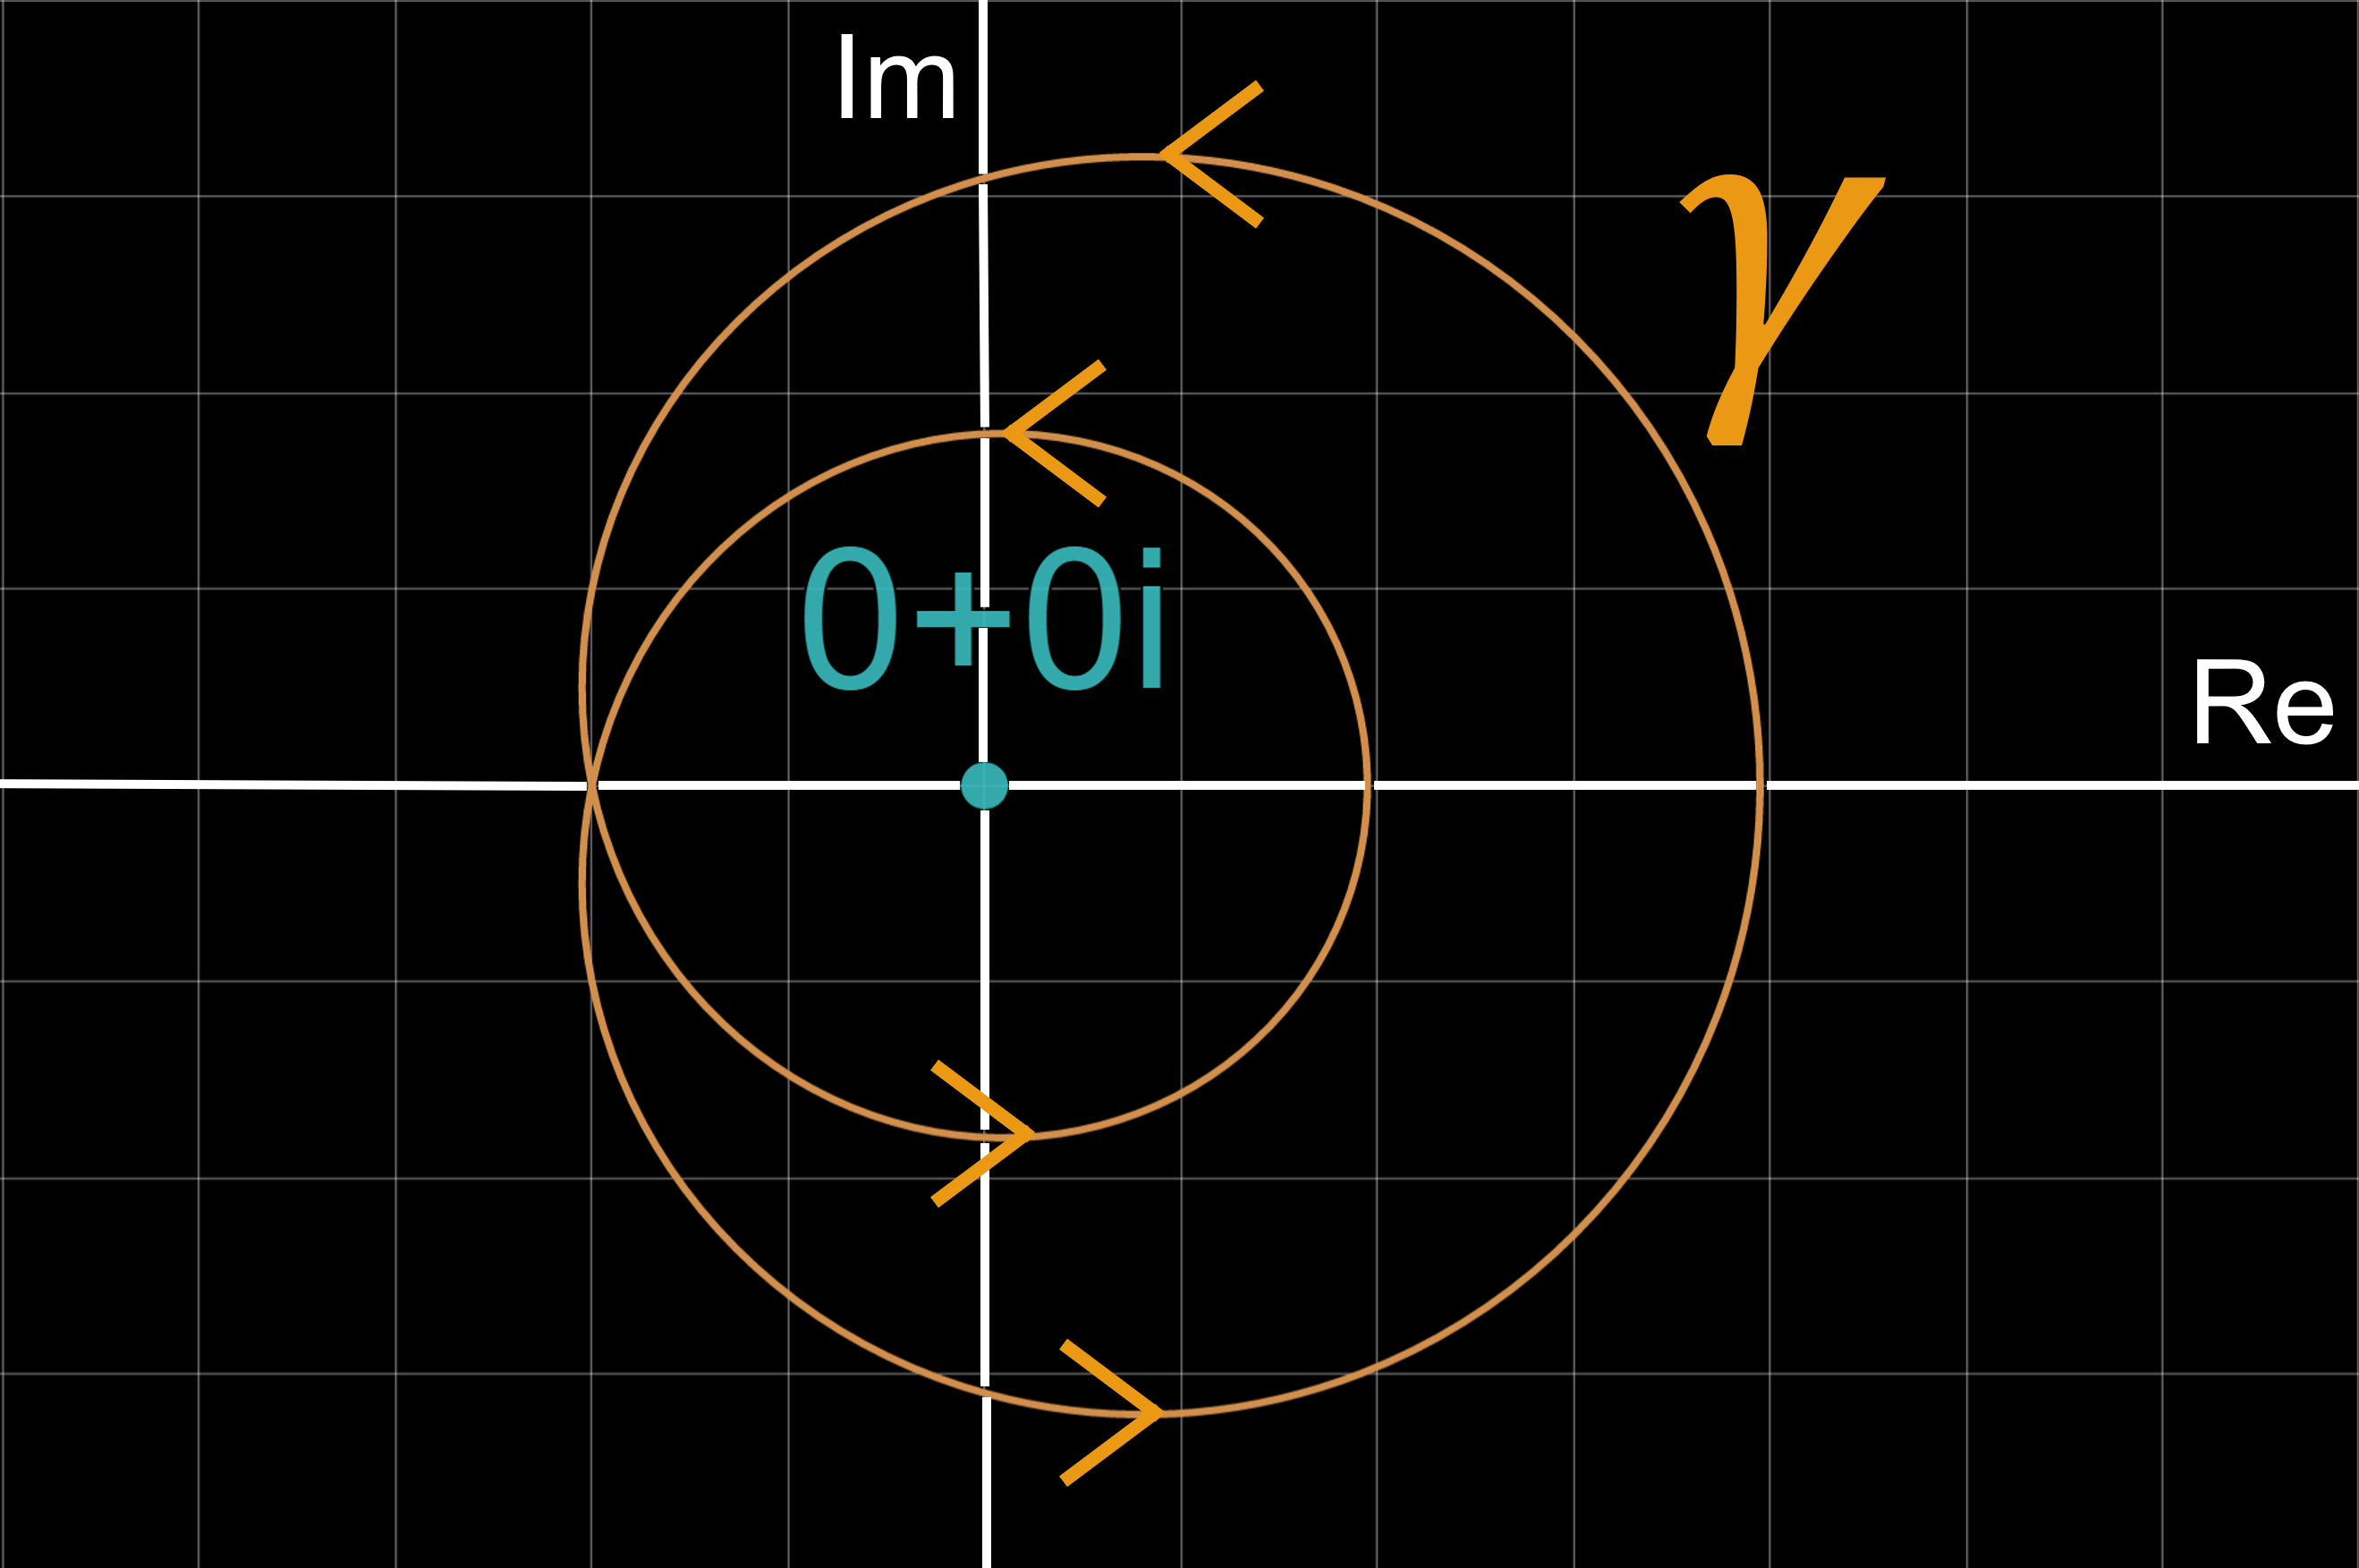
\includegraphics[scale=0.11]{limaconint4}
\end{center}
\end{example} 

\noindent\textit{Solution.}
From Example 5.1 we know that the only singularity is at $z=0$, and $\Res (f,0)= 1$, so all we have to do now is figure out the winding number at the singularity. Using the visualisation of $\gamma$ above, tracing the curve around the singularity shows that it revolves around it twice anticlockwise, so $W(\gamma,0)=2$. From there we use the residue theorem to compute 
\begin{align} 
\int_\gamma { f(\hat{z}) \dd\hat{z}} &= 2 \pi i \sum_{w \in \Phi} \Wind (\gamma,w) \Res (f,w) \nonumber \\
&= 2\pi i \Wind (\gamma,0) \Res (f,0) \nonumber \\
&= 4\pi i. \nonumber
\end{align}

So we have evaluated the contour integral around $e^{\nicefrac{1}{z}}$ for a self-intersecting curve, in what is a remarkably simple solution. Many similar integrals through self-intersecting contours are now solvable with this stronger version of the residue theorem.

\subsection{Further Applications of the Residue Theorem}

Now let us take a look at applications of the residue theorem - what makes this result useful?


\subsubsection{The Basel Problem}

The Basel Problem is a famous number theory problem, concocted by Pietro Mengoli (see \citep[p.1071]{BaselHist}) and solved by Leonard Euler in 1734 (see \citep[p.1067-1069]{BaselHist}). It states that

\[\sum_{j=1}^{\infty} \frac{1}{j^{2}} = \frac{\pi ^ {2}}{6}. \]



Euler used properties of finite polynomials and extended them to polynomials with infinite terms to solve this problem (an assumption at the time which was validated numerically), but an alternative proof using the residue theorem (see \citep[p.1, 6-7]{Basel}) is expressed concisely in this heuristic proof:
 
\begin{hproof}
Let $f(z) = \nicefrac{\pi \cot (\pi z)}{z^{2}}$. We observe that there are poles at every integer since $\cot (\pi z)$ will diverge at integer values of $z$. We create a square contour $\gamma$ oriented anticlockwise with vertices at $\pm (N+ \nicefrac{1}{2}) \pm i (N+ \nicefrac{1}{2})$ for $N \in \mathbb{Z}$.
We can note for all $N$, 
\[ \Wind (\gamma,0) \Res (f,0) + 2 \sum_{n=1}^{N} \Wind (\gamma,n) \Res (f,n) = \frac{1}{2 \pi i}\int_\gamma { \frac{\pi \cot (\pi \hat{z})}{\hat{z}^{2}} \dd\hat{z}}.\]
We calculate that the residue at $0$ is $\nicefrac{-\pi ^ {2}}{3}$ and the residue at $n$ is $\nicefrac{1}{n^{2}}$ for $n \in \mathbb{Z} \setminus \{0\}$. Since we used an anticlockwise square contour, the winding number of all terms will be $1$, and as $N \to \infty$, we can deduce
\[\sum_{n=1}^{\infty} \Res (f,n) = \sum_{n=1}^{\infty} \frac{1}{n^{2}} = \frac{1}{4 \pi i}\int_\gamma { \frac{\pi \cot (\pi \hat{z})}{\hat{z}^{2}} \dd\hat{z}} - \frac{1}{2} \Res (f,0) = \frac{\pi ^ {2}}{6}, \]
after showing the contour integral evaluates to $0$, using the fact that $\cot(\pi z)$ is bounded in $\gamma$.
\end{hproof}

\subsubsection{Calculating Inductance}

Inductance is the proclivity for an electrical conductor to oppose a change in flowing electrical current. Ampere's law describes the relationship between this current and magnetic fields as a line integral:
\[\oint_{\gamma}\mathbf{M} \cdot \dd \mathbf{r} = \mu_{0}I,\]
where $I$ is the net current enclosed by $\gamma$  (see \citep[p.2-3]{Magnets}). If we focus on a 2-dimensional case of Ampere's law, we can connect the result to the residue theorem. For $z=x+iy$, let $f(z) = \text{M}_{x} - i\text{M}_{y}$, then
\[\int_{\gamma} f(\hat{z}) \dd \hat{z} - i\oint_{\gamma} \text{M}_{\hat{x}} \dd \hat{x} - \text{M}_{\hat{y}} \dd \hat{y}= \oint_{\gamma} \text{M}_{\hat{x}} \dd \hat{x} + \text{M}_{\hat{y}} \dd \hat{y} = \oint_{\gamma}\mathbf{M} \cdot \dd \mathbf{r}.\]
The imaginary part of the integral is proportional to the $z$-component of a Lorentz force on a charge. If a charge travels with a constant current through $\gamma$, the magnetic field $\mathbf{M}$ will be parallel or anti parallel to the charge's motion, meaning there will be no force in the $z$ direction, giving us an intuitive reason for the imaginary integral to evaluate to $0$. We are then left with
\[\int_{\gamma} f(\hat{z}) \dd \hat{z} = \oint_{\gamma}\mathbf{M} \cdot \dd \mathbf{r} \implies 2 \pi i \sum_{w \in \Phi} \Wind (\gamma,w) \Res (f,w) = \mu_{0}I, \]
giving us an alternative method of calculating inductance, assuming $f(z)$ and $\gamma$ follow the conditions we proposed in Theorem 5.1.

\section{Conclusion}

The aim I set was to expand the residue theorem to account for not just simple but also self-intersecting contours that are valid for Cauchy's theorem regardless of orientation. We now have the ability to use any closed curve applicable to Cauchy's theorem for any function in which the singularities do not intersect with the curve - this is already useful as we have seen in Example 5.2, a contour integral we were not able to compute previously. 

However, we have not defined a case where our applicable curves actually intersect with singularities: what happens if singularities lie on the contour?

Only the winding number would be affected in this case, whereas the residue of the point would remain the same. We could intuitively say the winding number of a point on the contour - where the contour does not cross over itself - would be the arithmetic mean of the winding numbers of the 2 components it was connected to: if we think back to our tree rope analogy, we would end up on the opposite side of the tree after tracing through the contour, so we would get a winding number of $\nicefrac{(2n+1)}{2 }$, $n \in \mathbb{Z}$. 

However, not only is this conjecture and not mathematically robust, it also does not consider points in which a path crosses over itself, for which the winding number is intuitively unclear as we could traverse around the point both clockwise and anticlockwise. This is a possible area to research in the future.


\pagebreak
\bibliography{ResidueTheorem}

\end{document}
